\documentclass[11pt,twoside,a4paper]{article}
% http://www-h.eng.cam.ac.uk/help/tpl/textprocessing/latex_maths+pix/node6.html symboles de math
% http://fr.wikibooks.org/wiki/Programmation_LaTeX Programmation latex (wikibook)
%=========================== En-Tete =================================
%--- Insertion de paquetages (optionnel) ---
\usepackage[french]{babel}   % pour dire que le texte est en fran{\'e}ais
\usepackage{a4}	             % pour la taille   
\usepackage[T1]{fontenc}     % pour les font postscript
\usepackage{epsfig}          % pour gerer les images
%\usepackage{psfig}
\usepackage{amsmath, amsthm} % tres bon mode mathematique
\usepackage{amsfonts,amssymb}% permet la definition des ensembles
\usepackage{float}           % pour le placement des figure
\usepackage{verbatim}

\usepackage{longtable} % pour les tableaux de plusieurs pages

\usepackage[table]{xcolor} % couleur de fond des cellules de tableaux

\usepackage{lastpage}

% \usepackage[top=1.5cm, bottom=1.5cm, left=1.5cm, right=1.5cm]{geometry}
% gauche, haut, droite, bas, entete, ente2txt, pied, txt2pied
\usepackage{vmargin}
\setmarginsrb{1.0cm}{1.0cm}{1.0cm}{1.0cm}{15pt}{3pt}{60pt}{20pt}

\usepackage{lscape} % changement orientation page
%\usepackage{frbib} % enlever pour obtenir references en anglais
% --- style de page (pour les en-tete) ---
\pagestyle{headings}

% % % en-tete et pieds de page configurables : fancyhdr.sty

% http://www.trustonme.net/didactels/250.html

% http://ww3.ac-poitiers.fr/math/tex/pratique/entete/entete.htm
% http://www.ctan.org/tex-archive/macros/latex/contrib/fancyhdr/fancyhdr.pdf
\usepackage{fancyhdr}
\pagestyle{fancy}
% \newcommand{\chaptermark}[1]{\markboth{#1}{}}
% \newcommand{\sectionmark}[1]{\markright{\thesection\ #1}}
\fancyhf{}
\fancyhead[LE,RO]{\bfseries\thepage}
\fancyhead[LO]{\bfseries\rightmark}
\fancyhead[RE]{\bfseries\leftmark}
\fancyfoot[LE]{\thepage /\pageref{LastPage} \hfill
	JSON
\hfill 
\includegraphics[width=0.5cm]{img/logo_glider.png} }
\fancyfoot[RO]{
\includegraphics[width=0.5cm]{img/logo_glider.png} \hfill
	JSON
\hfill \thepage /\pageref{LastPage}}
\renewcommand{\headrulewidth}{0.5pt}
\renewcommand{\footrulewidth}{0.5pt}
\addtolength{\headheight}{0.5pt}
\fancypagestyle{plain}{
	\fancyhead{}
	\renewcommand{\headrulewidth}{0pt}
}

%% \pagestyle{empty}

\renewcommand{\headrulewidth}{0.25pt}
\renewcommand{\footrulewidth}{0.5pt}
%% \setlength{\headheight}{85pt}
% \addtolength{\headheight}{0.5pt}
% \fancypagestyle{plain}{
% 	\fancyhead{}
% 	\fancyfoot{}
% 	\renewcommand{\headrulewidth}{0pt}
% }

%--- Definitions de nouvelles commandes ---
\newcommand{\N}{\mathbb{N}} % les entiers naturels


%--- Pour le titre ---
\def\maketitle{%
	\begin{center}
		\begin{tabular}[c]{c|c}
			\textsc{\textbf{Institution}}~\\[\baselineskip]~\\[\baselineskip]
			\emph{\textbf{Date 09-09-2009}}~\\[\baselineskip]~\\[\baselineskip]
			\emph{\textbf{Pr{\'e}cisions relatives au contexte}}~\\[\baselineskip]~\\[\baselineskip]
			\textsc{Auteur inestimable}~\\[\baselineskip]~\\[\baselineskip]
			& 
			
\includegraphics[width=3cm]{img/logo_glider.png}~\\[\baselineskip]
		\end{tabular}
		% \\ \hline
		 	% % if more than one logo
			% 
\includegraphics[width=5cm]{img/logo_glider.png}
			% \includegraphics[width=5cm]{img/logo_wifi.png}
		% \\ \hline
		% \end{tabular}
			~\\[\baselineskip]~\\[\baselineskip]
			\Huge{Titre principal}~\\[\baselineskip]
			\Large{Titre secondaire}~\\[\baselineskip]
		
		~\\[\baselineskip]
		~\\[\baselineskip]
	\large{
		\textsc{\textbf{Institution d'accueil et jury}}
		~\\[\baselineskip]
		<<titre personne>> : \texttt{Anne ONYME}~\\[\baselineskip]
		<<titre personne>> : \texttt{Jocelyn CONNU}~\\[\baselineskip]
		~\\[\baselineskip]
		\textit{Pr{\'e}cisions du contexte de r{\'e}daction de l'article}
	}

	\end{center}

}%



%--- Pour le glossaire --- a defaut de \makeglossary ou d'utilisation d'index latex

\definecolor{verylightgray}{rgb}{0.8,0.8,0.8}
\def\makeglossaire{%
	\begin{center}

	\begin{tabular}{|>{\columncolor{verylightgray}} p{0.2\textwidth}|p{0.8\textwidth}|}

		\hline

		\textbf{BLAST} & 

			\begin{tabular}{p{0.8\textwidth}}

			Basic Local Alignment Search Tool \\

			\textit{algorithmes et logiciels pour l'alignement de s{\'e}quences et la recherche de similarit{\'e}s locales}

			\end{tabular} \\

		\hline

		\textbf{BNDB} & Biochemical NetWork DataBase \textit{(entrep{\^o}t de donn{\'e}es)} \\

		\hline

	\end{tabular}

\end{center}

}%

%============================= Corps =================================
\begin{document}
%ecrire le titre...
%% \maketitle
%% \setcounter{page}{0}
%% \thispagestyle{empty}
%% \clearpage

%% \setcounter{page}{0}
%% \thispagestyle{empty}

\setlength\parindent{0pt}

\texttt{\small http://www.json.org/ }~\\

\textbf{\Large JSON}~\\
\emph{ --- }~\\

\textbf{JSON} (JavaScript Object Notation) is a lightweight data-interchange format. It is easy for humans to read and write. It is easy for machines to parse and generate. It is based on a subset of the JavaScript Programming Language, Standard ECMA-262 3rd Edition - December 1999. JSON is a text format that is completely language independent but uses conventions that are familiar to programmers of the C-family of languages, including C, C++, C\#, Java, JavaScript, Perl, Python, and many others. These properties make JSON an ideal data-interchange language. ~\\

JSON is built on two structures:
\begin{itemize}
	\item A collection of name/value pairs. In various languages, this is realized as an object, record, struct, dictionary, hash table, keyed list, or associative array.
    \item An ordered list of values. In most languages, this is realized as an array, vector, list, or sequence.
\end{itemize}

These are universal data structures. Virtually all modern programming languages support them in one form or another. It makes sense that a data format that is interchangeable with programming languages also be based on these structures.~\\

In JSON, they take on these forms:~\\

%% \begin{minipage}[h]{0.75\textwidth}
%% 	\includegraphics[width=0.95\textwidth]{img/L17_Blockchain258_0.jpg}
%% \end{minipage} \hfill \begin{minipage}[h]{0.23\textwidth}
%% 	Cette technologie rappelle les facteurs de disruption tels qu'Uber, puisqu'elle repose sur les m{\^e}mes principes de d{\'e}centralisation, de partage et d'utilisation d'Internet. Mais elle est r{\'e}volutionnaire, puisqu'elle concernera toutes les branches qui font appel {\`a} un interm{\'e}diaire. Elle int{\`e}gre aussi les facteurs de tra\c{c}abilit{\'e} des informations et de d{\'e}centralisation. ~\\
%% \end{minipage} ~\\~\\

	An \emph{object} is an unordered set of name/value pairs. An object begins with \{$_{(left brace)}$ and ends with \}$_{(right brace)}$. Each name is followed by :$_{(colon)}$ and the name/value pairs are separated by ,$_{(comma)}$.~\\
	
	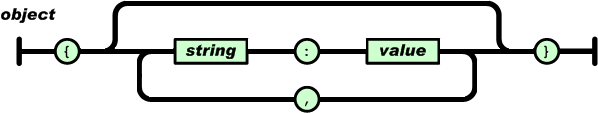
\includegraphics[width=0.95\textwidth]{img/object.png}~\\
	
	An \emph{array} is an ordered collection of values. An array begins with [$_{(left bracket)}$ and ends with ]$_{(right bracket)}$. Values are separated by ,$_{(comma)}$.~\\
	
	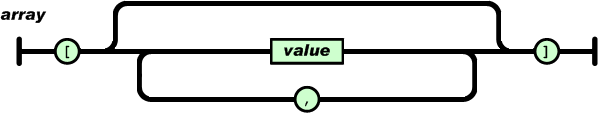
\includegraphics[width=0.95\textwidth]{img/array.png}~\\

\begin{minipage}[h]{0.70\textwidth}
	\small
	A \emph{value} can be a string in double quotes, or a number, or true or false or null, or an object or an array. These structures can be nested.~\\
	
	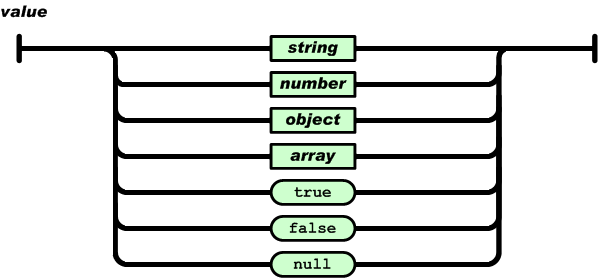
\includegraphics[width=0.95\textwidth]{img/value.png}~\\
	
	A \emph{string} is a sequence of zero or more Unicode characters, wrapped in double quotes, using backslash escapes. A character is represented as a single character string. A string is very much like a C or Java string.~\\
	
	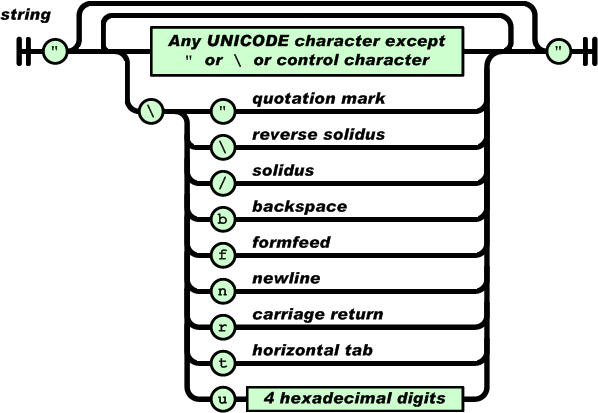
\includegraphics[width=0.95\textwidth]{img/string.png}~\\
	
	A \emph{number} is very much like a C or Java number, except that the octal and hexadecimal formats are not used.~\\
	
	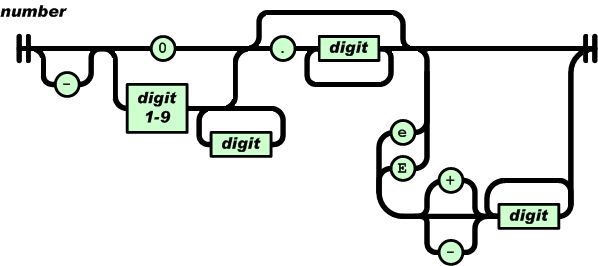
\includegraphics[width=0.95\textwidth]{img/number.png}~\\
	
	Whitespace can be inserted between any pair of tokens. Excepting a few encoding details, that completely describes the language.~\\

\end{minipage} \hfill \begin{minipage}[h]{0.30\textwidth}
	\footnotesize
	\begin{itemize}
		\item[] object
		\begin{itemize}
			\item[] \{\} ; \{ members \}
		\end{itemize} 
		\item[] members
		\begin{itemize}
			\item[] pair
			\item[] pair , members
		\end{itemize}
		\item[] pair
		\begin{itemize}
			\item[] string : value
		\end{itemize}
		\item[] array
		\begin{itemize}
			\item[] [] ; [ elements ]
		\end{itemize}
		\item[] elements
		\begin{itemize}
			\item[] value
			\item[] value , elements
		\end{itemize}
		\item[] value
		\begin{itemize}
			\item[] string ; number ; 
			\item[] object ; array ;
			\item[] true ; false ;
			\item[] null
		\end{itemize}
		\item[] string
		\begin{itemize}
			\item[] "" ; " chars "
		\end{itemize}
		\item[] chars
		\begin{itemize}
			\item[] char
			\item[] char chars
		\end{itemize}
		\item[] char
		\begin{itemize}
			\item[] any-Unicode-character-
			\begin{itemize}
				\item[] except-"-or-$\backslash \backslash$-or-
				\item[] control-character
			\end{itemize}
			\item[] $\backslash "$ ; $\backslash \backslash$ ; $\backslash /$ ; $\backslash b$ ; $\backslash f$ ; $\backslash n$ ; $\backslash r$ ; $\backslash t$ ; $\backslash u$ four-hex-digits
		\end{itemize} 
		\item[] number
		\begin{itemize}
			\item[] int
			\item[] int frac
			\item[] int exp
			\item[] int frac exp
		\end{itemize} 
		\item[] int
		\begin{itemize}
			\item[] digit
			\item[] digit1-9 digits
			\item[] -- digit
			\item[] -- digit1-9 digits
		\end{itemize} 
		\item[] frac
		\begin{itemize}
			\item[] . digits
		\end{itemize}
		\item[] exp
		\begin{itemize}
			\item[] e digits
		\end{itemize}
		\item[] digits
		\begin{itemize}
			\item[] digit
			\item[] digit digits
		\end{itemize}
		\item[] e
		\begin{itemize}
			\item[] e ; e+ ; e-
			\item[] E ; E+ ; E-
		\end{itemize}
	\end{itemize}~\\

\end{minipage}

\end{document}
